\documentclass[aspectratio=169,10pt]{ctexbeamer}

\usetheme{Madrid}
\usecolortheme{default}
\setbeamertemplate{navigation symbols}{}
\setbeamertemplate{footline}[frame number]

\usepackage{amsmath}
\usepackage{booktabs}
\usepackage{array}
\usepackage{graphicx}
\usepackage{tikz}
\usepackage{xcolor}
\usepackage{listings}
\usetikzlibrary{arrows.meta, positioning}

\definecolor{ucasblue}{RGB}{30,70,120}
\definecolor{ucasgreen}{RGB}{36,120,92}
\definecolor{lightgray}{RGB}{245,247,250}
\definecolor{codeblue}{RGB}{28,68,135}
\definecolor{codegreen}{RGB}{40,120,80}

\setbeamercolor{structure}{fg=ucasblue}
\setbeamercolor{title}{fg=white,bg=ucasblue}
\setbeamercolor{frametitle}{fg=white,bg=ucasblue}
\setbeamercolor{block title}{fg=white,bg=ucasblue}
\setbeamercolor{block body}{bg=lightgray}
\setbeamerfont{frametitle}{series=\bfseries}
\setbeamerfont{title}{series=\bfseries,size=\Large}

\newcolumntype{M}[1]{>{\centering\arraybackslash}m{#1}}
\graphicspath{{../Figure/}}

\lstset{
	language=Python,
	basicstyle=\ttfamily\scriptsize,
	numbers=left,
	numberstyle=\tiny\color{ucasgreen},
	showstringspaces=false,
	breaklines=true,
	frame=single,
	rulecolor=\color{ucasblue!45},
	framerule=0.4pt,
	backgroundcolor=\color{lightgray},
	columns=fullflexible,
	keywordstyle=\bfseries\color{codeblue},
	commentstyle=\itshape\color{codegreen},
	stringstyle=\color{red!65!black},
	tabsize=4
}

\title{实验一：手写数字识别}
\subtitle{基于卷积神经网络的 MNIST 分类}
\author{尧祥临 \quad 202518023406038}
\institute{中国科学院大学 \quad 前沿交叉科学学院\\2026年春季学期\quad 深度学习}
\date{}

\begin{document}

\begin{frame}
	\titlepage
\end{frame}

\begin{frame}{实验任务}
	\begin{block}{目标}
		在 MNIST 手写数字数据集上构建并训练卷积神经网络，实现 0 到 9 共 10 类数字图象分类。
	\end{block}

	\begin{columns}[T,onlytextwidth]
		\begin{column}{0.48\textwidth}
			\textbf{实验要求}
			\begin{itemize}
				\item 使用 PyTorch 完成数据加载、模型构建与训练
				\item 搭建规范的 CNN 网络结构
				\item 测试集准确率达到 98\% 及以上
			\end{itemize}
		\end{column}
		\begin{column}{0.48\textwidth}
			\textbf{本次完成情况}
			\begin{itemize}
				\item 训练 20 个 epoch
				\item 保存训练日志和模型参数
				\item 最终测试集准确率：\textbf{99.33\%}
			\end{itemize}
		\end{column}
	\end{columns}
\end{frame}

\begin{frame}{数据集与划分}
	\begin{columns}[T,onlytextwidth]
		\begin{column}{0.52\textwidth}
			\begin{itemize}
				\item 数据集：MNIST 手写数字数据集
				\item 输入尺寸：$1\times 28\times 28$ 灰度图象
				\item 类别数：10 类，对应数字 0 到 9
				\item 输入预处理：\texttt{transforms.ToTensor()}
			\end{itemize}
		\end{column}
		\begin{column}{0.43\textwidth}
			\begin{table}
				\centering
				\begin{tabular}{l r}
					\toprule
					划分 & 样本数 \\
					\midrule
					训练集 & 55000 \\
					验证集 & 5000 \\
					测试集 & 10000 \\
					\bottomrule
				\end{tabular}
			\end{table}
		\end{column}
	\end{columns}

	\vspace{0.2cm}
	\begin{block}{划分方式}
		从原始 60000 张训练图象中随机划分 55000 张用于训练，5000 张用于验证；测试集保持官方 10000 张不变。
	\end{block}
\end{frame}

\begin{frame}{整体流程}
	\centering
	\begin{tikzpicture}[
		node distance=0.55cm,
		flowstep/.style={draw=ucasblue, fill=lightgray, rounded corners=2pt,
			minimum width=2.5cm, minimum height=0.8cm, align=center},
		arrow/.style={-{Latex[length=2.2mm]}, thick, draw=ucasblue}
	]
		\node[flowstep] (data) {加载 MNIST\\构建 DataLoader};
		\node[flowstep, right=of data] (model) {定义 CNN\\前向传播};
		\node[flowstep, right=of model] (loss) {交叉熵损失\\AdamW 优化};
		\node[flowstep, right=of loss] (train) {训练与验证\\记录日志};
		\node[flowstep, right=of train] (eval) {测试评估\\保存模型};

		\draw[arrow] (data) -- (model);
		\draw[arrow] (model) -- (loss);
		\draw[arrow] (loss) -- (train);
		\draw[arrow] (train) -- (eval);
	\end{tikzpicture}

	\vspace{0.8cm}
	\begin{columns}[T,onlytextwidth]
		\begin{column}{0.5\textwidth}
			\textbf{训练阶段}
			\begin{itemize}
				\item \texttt{model.train()}
				\item 前向传播、反向传播、参数更新
			\end{itemize}
		\end{column}
		\begin{column}{0.45\textwidth}
			\textbf{评估阶段}
			\begin{itemize}
				\item \texttt{model.eval()}
				\item 计算 loss 和 accuracy
			\end{itemize}
		\end{column}
	\end{columns}
\end{frame}

\begin{frame}{CNN 模型结构}
	\centering
	\resizebox{\linewidth}{!}{%
	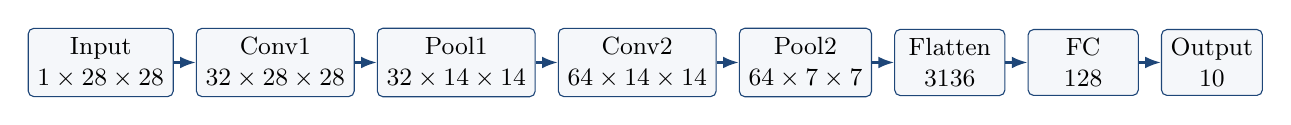
\begin{tikzpicture}[
		layer/.style={draw=ucasblue, fill=lightgray, rounded corners=2pt,
			minimum height=0.75cm, align=center, font=\small},
		arrow/.style={-{Latex[length=2mm]}, thick, draw=ucasblue},
		node distance=0.28cm
	]
		\node[layer, minimum width=1.4cm] (input) {Input\\$1\times28\times28$};
		\node[layer, minimum width=1.5cm, right=of input] (conv1) {Conv1\\$32\times28\times28$};
		\node[layer, minimum width=1.4cm, right=of conv1] (pool1) {Pool1\\$32\times14\times14$};
		\node[layer, minimum width=1.5cm, right=of pool1] (conv2) {Conv2\\$64\times14\times14$};
		\node[layer, minimum width=1.4cm, right=of conv2] (pool2) {Pool2\\$64\times7\times7$};
		\node[layer, minimum width=1.4cm, right=of pool2] (flat) {Flatten\\3136};
		\node[layer, minimum width=1.4cm, right=of flat] (fc) {FC\\128};
		\node[layer, minimum width=1.2cm, right=of fc] (out) {Output\\10};

		\foreach \a/\b in {input/conv1,conv1/pool1,pool1/conv2,conv2/pool2,pool2/flat,flat/fc,fc/out}
			\draw[arrow] (\a) -- (\b);
	\end{tikzpicture}
	}

	\vspace{0.55cm}
	\begin{columns}[T,onlytextwidth]
		\begin{column}{0.48\textwidth}
			\begin{block}{卷积与池化}
				两个卷积层均采用 $5\times5$ 卷积核、stride 1、padding 2；最大池化采用 $2\times2$、stride 2。
			\end{block}
		\end{column}
		\begin{column}{0.48\textwidth}
			\begin{block}{分类头}
				将 $64\times7\times7$ 特征图展平为 3136 维向量，经过 128 维隐藏层后输出 10 类 logits。
			\end{block}
		\end{column}
	\end{columns}
\end{frame}

\begin{frame}[fragile]{模型核心代码}
\begin{lstlisting}
class CNN(nn.Module):
    def __init__(self, hidden_dim=128):
        super(CNN, self).__init__()
        self.conv1 = nn.Conv2d(1, 32, kernel_size=5, stride=1, padding=2)
        self.relu1 = nn.ReLU()
        self.pool1 = nn.MaxPool2d(kernel_size=2, stride=2)

        self.conv2 = nn.Conv2d(32, 64, kernel_size=5, stride=1, padding=2)
        self.relu2 = nn.ReLU()
        self.pool2 = nn.MaxPool2d(kernel_size=2, stride=2)

        self.fc = nn.Sequential(
            nn.Flatten(),
            nn.Linear(64 * 7 * 7, hidden_dim),
            nn.ReLU(),
            nn.Linear(hidden_dim, 10)
        )

    def forward(self, x):
        x = self.pool1(self.relu1(self.conv1(x)))
        x = self.pool2(self.relu2(self.conv2(x)))
        return self.fc(x)
\end{lstlisting}
\end{frame}

\begin{frame}{参数量与尺寸变化}
	\begin{columns}[T,onlytextwidth]
		\begin{column}{0.54\textwidth}
			\begin{table}
				\centering
				\small
				\begin{tabular}{l c c}
					\toprule
					层 & 输出尺寸 & 参数量 \\
					\midrule
					Conv1 & $32\times28\times28$ & 832 \\
					Conv2 & $64\times14\times14$ & 51264 \\
					Linear1 & 128 & 401536 \\
					Linear2 & 10 & 1290 \\
					\midrule
					总计 & -- & 454922 \\
					\bottomrule
				\end{tabular}
			\end{table}
		\end{column}
		\begin{column}{0.42\textwidth}
			\begin{block}{尺寸计算}
				\[
					H_{\mathrm{out}}=
					\left\lfloor\frac{H_{\mathrm{in}}+2P-K}{S}\right\rfloor+1
				\]
			\end{block}
			\begin{itemize}
				\item padding 2 保持卷积前后尺寸不变
				\item 两次最大池化将 $28\rightarrow14\rightarrow7$
				\item 参数主要集中在第一个全连接层
			\end{itemize}
		\end{column}
	\end{columns}
\end{frame}

\begin{frame}{训练配置}
	\begin{columns}[T,onlytextwidth]
		\begin{column}{0.48\textwidth}
			\begin{table}
				\centering
				\small
				\begin{tabular}{l l}
					\toprule
					项目 & 设置 \\
					\midrule
					Batch size & 64 \\
					Epochs & 20 \\
					Learning rate & $5\times10^{-4}$ \\
					隐藏层维度 & 128 \\
					优化器 & AdamW \\
					损失函数 & CrossEntropyLoss \\
					训练设备 & CUDA GPU \\
					\bottomrule
				\end{tabular}
			\end{table}
		\end{column}
		\begin{column}{0.47\textwidth}
			\begin{block}{损失函数}
				\[
					\mathcal{L}=-\frac{1}{B}\sum_{i=1}^{B}
					\log \frac{\exp(z_{i,y_i})}{\sum_{c=0}^{9}\exp(z_{i,c})}
				\]
			\end{block}
			\begin{itemize}
				\item 每个 epoch 后记录验证集和测试集指标
				\item 训练日志保存为 \texttt{train\_log.csv}
				\item 模型参数保存为 \texttt{cnn\_mnist.pth}
			\end{itemize}
		\end{column}
	\end{columns}
\end{frame}

\begin{frame}{训练结果}
	\begin{table}
		\centering
		\small
		\begin{tabular}{M{1.2cm} M{1.7cm} M{1.7cm} M{1.7cm} M{1.7cm} M{1.7cm}}
			\toprule
			Epoch & Train Loss & Val Loss & Val Acc & Test Loss & Test Acc \\
			\midrule
			1  & 0.2084 & 0.0680 & 97.78\% & 0.0518 & 98.32\% \\
			5  & 0.0235 & 0.0384 & 98.80\% & 0.0321 & 98.86\% \\
			10 & 0.0087 & 0.0326 & 99.18\% & 0.0308 & 99.19\% \\
			15 & 0.0031 & 0.0319 & 99.14\% & 0.0297 & 99.23\% \\
			19 & 0.0026 & 0.0267 & 99.32\% & 0.0310 & 99.31\% \\
			20 & 0.0022 & 0.0289 & 99.20\% & 0.0312 & \textbf{99.33\%} \\
			\bottomrule
		\end{tabular}
	\end{table}

	\begin{block}{观察}
		第 1 个 epoch 后测试准确率已经达到 98.32\%，超过实验要求；训练到第 20 个 epoch 后测试准确率提升到 99.33\%。
	\end{block}
\end{frame}

\begin{frame}{训练曲线}
	\centering
	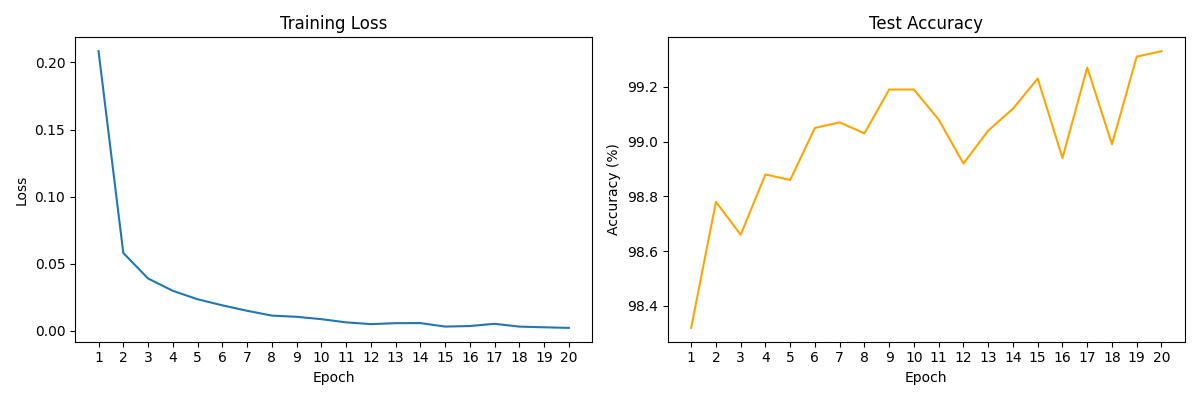
\includegraphics[width=0.88\linewidth]{train_log.png}

	\vspace{0.25cm}
	\begin{itemize}
		\item 训练损失在前几个 epoch 快速下降，随后逐渐收敛
		\item 测试准确率整体位于 99\% 附近并继续提升
		\item 第 16 个 epoch 附近存在一次波动，但后续恢复到较低 loss 和较高 accuracy
	\end{itemize}
\end{frame}

\begin{frame}{结果分析}
	\begin{columns}[T,onlytextwidth]
		\begin{column}{0.49\textwidth}
			\begin{block}{模型有效性}
				两层卷积能够提取局部笔画、边缘和组合模式；对 MNIST 这种规整的灰度分类任务，浅层 CNN 已经具备较强表达能力。
			\end{block}
		\end{column}
		\begin{column}{0.49\textwidth}
			\begin{block}{泛化表现}
				训练后期验证集和测试集准确率保持在 99\% 左右，没有出现持续恶化的过拟合趋势。
			\end{block}
		\end{column}
	\end{columns}

	\vspace{0.4cm}
	\begin{itemize}
		\item 最终测试准确率：\textbf{99.33\%}
		\item 实验要求：测试准确率不低于 98\%
		\item 模型文件：\texttt{Lab1/model/cnn\_mnist.pth}
	\end{itemize}
\end{frame}

\begin{frame}{总结}
	\begin{block}{完成内容}
		本次实验基于 PyTorch 完成了 MNIST 手写数字识别，包括数据加载与划分、CNN 模型搭建、训练评估、日志记录、模型保存和结果可视化。
	\end{block}

	\begin{block}{主要收获}
		进一步熟悉了卷积、激活、池化和全连接分类头的配合方式，也掌握了 \texttt{Dataset}、\texttt{DataLoader}、\texttt{nn.Module}、反向传播和优化器更新的基本流程。
	\end{block}

	\begin{block}{可改进方向}
		固定随机种子增强复现性；加入输入标准化；补充混淆矩阵，分析不同数字类别之间的错误模式。
	\end{block}
\end{frame}

\end{document}
